\documentclass[../thesis]{subfiles}
\graphicspath{{\subfix{../figures/}}}

\begin{document}
\chapter{User Study}\label{ch:evaluation}

\lettrine[lines=3]{\textcolor{Maroon}{D}}{espite} having already done a technical evaluation in \cref{sec:techeval}, it is usually also a good idea to compare new approaches with existing state-of-the-art tools in a user study.
In our case, we want to compare \SEE{}'s \gls{lsp}-generated \glspl{city} with the \glspl{capability} a normal \gls{lsp}-enabled \gls{ide} offers.
For the latter, the Microsoft-developed \gls{ide} \gls{vscode} is a good fit, given that the \glsentrylong{lsp} itself originates here (see \cref{sec:lsp}) and that it still has a deep integration with it.

First, we will outline the general aim of this study by going over some existing related research, explaining important aspects of \gls{vscode}, and then enumerating our hypotheses.
Next, we will explain the details of the design of the study itself, before analyzing its results with the \participants{} participants in detail.
Finally, we describe some relevant threats to validity.

As a quick aside before we begin, we will frequently use \glspl{violin} in this chapter to visualize datasets, especially to visually compare two datasets against one another.
To estimate the probability density for the plots, we need to use a non-parametric kernel density estimation (since we do not know which shape the underlying distribution has)---for the kernel itself, we simply use a gaussian function, but a much more important question is the choice of the bandwidth parameter~\cite{heidenreich2013}.
Here, we use an algorithm by \textcite{sheather1991} that has been improved to be made more performant and handle multimodal distributions better by \textcite{botev2010a}:
The \emph{Improved Sheather--Jones} method, which is a robust choice when one cannot assume normality~\cite{akinshin2020}.
As the algorithm for this method, we use \tt{KDEpy}~\cite{odland2018}, whose implementation of the method is based on \textcite[326--328]{kroese2011}.
A drawback here is that this algorithm does not necessarily converge.
In those cases, we fall back to using Silverman's rule of thumb~\cite{silverman1986}, the implementation of which is integrated into the library we use to draw these plots~\cite{callil-soares2024}.

\section{Plan}\label{sec:plan}
Our main aim here is to answer our second research question that we defined in \cref{sec:goals}:
\begin{displayquote}
	Are \glspl{city} a suitable means to present \gls{lsp} information to developers as compared to \glspl{ide} + tables (on the dimensions of speed, accuracy, and usability)?
\end{displayquote}

To empirically evaluate this research question, we will devise a series of short software engineering related tasks on the real-world software projects \emph{JabRef}\footnote{
	\web{https://github.com/JabRef/jabref}{2024-11-22}
} and \emph{SpotBugs}\footnote{
	\web{https://github.com/spotbugs/spotbugs}{2024-11-22}
}.
Participants then get randomly assigned to either use \SEE{} (along with our implementation from \cref{ch:implementation}) or \gls{vscode} (with an active \gls{ls}).
However, evaluating the supported \glspl{capability} (see \cref{tab:capabilities}) in this way turns out to be quite difficult---for example, how would one evaluate the \emph{Hover} \gls{capability}, let alone features like \glspl{token} which are almost identically implemented across \SEE{} and \gls{vscode}?
For this reason, we will abstain from incorporating the \gls{window}-related \glspl{capability} from \cref{sec:intowindow}.
Limiting ourselves, then, to the \gls{city}-related changes from \cref{sec:intocity}, we have:
\begin{enumerate}
	\item \emph{Diagnostics} being displayed as erosion icons above corresponding nodes.
	      \begin{description}
		      \item[\follows{}] This feature was essentially already evaluated in my bachelor's thesis, albeit with the Axivion Dashboard as a data source instead of \gls{lsp}~\cite{galperin2021,galperin2022}.
	      \end{description}
	\item \emph{Hover} details being displayed when the user hovers the mouse above a node.
	      \begin{description}
		      \item[\follows{}] Since this is used here almost identically as in \glspl{window}, it does not make much sense to compare it against \gls{vscode}.
	      \end{description}
	\item \emph{Go to location}, \emph{references}, and \emph{call/type hierarchy} being used for rendered edges and context menu actions.
	      \begin{description}
		      \item[\follows{}] The context menu actions are not interesting to evaluate for the same reasons as above, though this does not apply to the generated edges.
	      \end{description}
\end{enumerate}

It appears that the only \glspl{capability} that are reasonably evaluable in a user study of this form are actually the ones used in the generation of the \gls{city} in \cref{sec:generate}.
Besides, the bulk of the implementation pertains to the generation of \glspl{city}, so it makes sense to focus on them here.
As a result, the user study is now actually of a form (directly comparing \glspl{city} against \glspl{ide}) that has been researched in previous literature before, so let us take a look at that research first before designing our own study.

\subsection{Existing Research}\label{subsec:research}
Across various bachelor's and master's theses, a number of user studies have been performed about \SEE{}'s usability in various aspects~\cite{davidwagner2020, felixgaebler2021, hannesmasuch2020, kevindoehl2020, maximilianwick2022, michelkrause2024, robertbohnsack2020, rubensmidt2021} as well as about its effectiveness compared to traditional tools~\cite{galperin2021, lennartkipka2020, moritz, nicoweiser2021, rohlfing2024, schramm2022, sulanabubakarov2021, yannisrohloff2021}.
Especially relevant among the latter kind of studies are the three that compare \SEE{} with traditional \glspl{ide}, as that is very close to our own planned evaluation.
Two of these evaluate debugging capabilities that have been implemented into \SEE{}:
\textcite{lennartkipka2020} compares those with Eclipse\footnote{
	\web{https://www.eclipse.org/}{2024-11-17}
}'s debugger, while \textcite{rohlfing2024} uses the debugger of \gls{vscode} as a baseline.
The final of these studies has \textcite{schramm2022} compare pure \gls{ide} usage (in this case, Microsoft's Visual Studio) with a combination of Visual Studio and \SEE{} in which Visual Studio has a plugin setup that integrates it with \SEE{}.
The result here was a significant improvement for usability and a partial improvement for efficiency in favor of the combination of Visual Studio and \SEE{}.
Almost all of these \SEE{}-related studies measure its usability in the form of the \gls{sus}---which we will do in our own study, as well.
I have collected the existing scores of those studies in a \gls{violin} in \cref{fig:seesus}.

\pgfplotsset{axis line style={draw=none}}

\begin{figure}
	\begin{center}
		\begin{tikzpicture}
			\violinsetoptions[data points,scaled,averages]{
				xmin=0,xmax=2,
				ymin=55,ymax=95,
				xticklabel style={yshift={-2cm}},
				ylabel={SUS},
				set layers,
				ymajorgrids=true,
				name=violin
			}

			\violinplot[%
				index=sus,%
				col sep=tab,%
				color=Maroon,%
				dataset size=3pt,%
				average size=5pt,%
				average opacity=0.8,%
				average color=black,%
				dataset opacity=0.8,%
				dataset jitter=0.1,%
				relative position=1,%
				bandwidth=2.1269,%
				average fill opacity=0.5,%
				average fill=ForestGreen,%
				average mark=otimes*,%
				dataset color=black,%
				dataset fill=black,%
				dataset fill opacity=0.5,%
				label={}
			]{analysis/dat/sus.dat}

			\node(xlabel) at ($(violin.south) + (0,-0.5)$) {\small \textcolor{Gray!50!Black}{SEE}};

			\plotornaments{violin}
		\end{tikzpicture}
	\end{center}
	\caption{\Gls{sus} results for \SEE{} across sixteen studies~\cite{davidwagner2020, felixgaebler2021, galperin2021, hannesmasuch2020, kevindoehl2020, lennartkipka2020, maximilianwick2022, michelkrause2024, moritz, nicoweiser2021, robertbohnsack2020, rohlfing2024, rubensmidt2021, schramm2022, sulanabubakarov2021, yannisrohloff2021}.}\label{fig:seesus}
\end{figure}

Outside of \SEE{}, there are a number of other \gls{city} implementations, such as \emph{CodeCity}~\cite{wettel2007} or \emph{Software World}~\cite{knight2000} (see also the overview by \textcite{jeffery2019}).
In their evaluations, these papers often compare different platforms (such as Desktop to VR/AR)~\cite[\eg,][]{merino2017,fittkau2015, merino2018}, but as with the \SEE{}-related theses above, we are most interested in those that have controlled experiments comparing a \gls{city} implementation with a traditional \gls{ide}.

One such study was done by \textcite{wettel2011} and compares \emph{CodeCity} against the Eclipse \gls{ide}, with the caveat that participants using Eclipse can also access an Excel spreadsheet of software metrics, as the \gls{city} implementation would otherwise have an unfair advantage.
He based his study on an extensive survey of existing empirical work on software visualization, constructing a "wishlist" of desiderata for such studies~\cite[chapter 7]{wettel2011}.
We will refer back to this wishlist, and to his experiment design in general, in \cref{sec:design} for our own study.
The study was later replicated by \textcite{romano2019} with a subset of tasks.

Similarly, \textcite{mortara2024} supplied \gls{csv} files for \gls{ide} users in a comparison against \emph{VariCity}, although here, participants were allowed to choose whatever \gls{ide} they are most comfortable with.
\textcite{mehra2020} gave participants who were using Eclipse an additional 2D graph tool when evaluating the augmented reality \textsc{XRaSE} \gls{city} visualization.
On the other hand, the category of comparative user studies between \glspl{city} and \glspl{ide} without any other helper tools includes ones by \textcite{khaloo2017,galperin2022,lennartkipka2020}.
The results of their experiments, and all others cited here, are listed in the color-coded \cref{tab:compresults}.

\colorlet{LightMaroon}{Maroon!30!white}
\colorlet{LightBlue}{Cyan!30!white}

% Maybe also for non-IDE comp for SEE?
% yellow: mixed, gray: no sig. diff., (light) maroon favor of CC, (light) blue: favor of IDE
% with legend

\newcommand{\reside}[1]{\cellcolor{Blue}\textcolor{White}{#1}}
\newcommand{\rescc}[1]{\cellcolor{Maroon}\textcolor{White}{#1}}
\newcommand{\residel}[1]{\cellcolor{LightBlue}#1}  % e.g., < 50% of tasks
\newcommand{\resccl}[1]{\cellcolor{LightMaroon}#1}
\newcommand{\resmixed}[1]{\cellcolor{Goldenrod}#1}  % Mixed between tasks
\newcommand{\resnone}[1]{\cellcolor{Gray!70!white}No diff.}  % No sig. diff.
% White: not measured
\newcommand{\resna}[1]{\textcolor{Gray}{\textit{N/A}}}

\begin{table}
	\begin{center}
		\caption{Results of various studies comparing \glspl{city} (CC) against \glspl{ide}. $x/y$ indicates an advantage in $x$ out of $y$ tasks or questions.}\label{tab:compresults}
		{
			\footnotesize
			\def\arraystretch{1.3}
			\begin{tabular}{|l|l|l|l|l|l|l|}
				\hline
				Study                   & $n$ & Correctness         & Time                           & Usability                      & \gls{ide}          & Code City      \\ \hline
				\cite{wettel2011}       & 45  & \rescc{$p = 0.001$} & \rescc{$p=0.043$}              & \resna{}                       & Eclipse + metrics  & CodeCity       \\ \hline
				\cite{khaloo2017}       & 28  & \resna{}            & \reside{$3/5$ IDE}             & \resccl{$6/20$ CC; $1/20$ IDE} & Visual Studio (VS) & Code Park      \\ \hline
				\cite{romano2019}       & 54  & \rescc{$p= 0.005$}  & \rescc{$p < 0.001\%$}          & \resnone{}                     & Eclipse + metrics  & Code2City      \\ \hline
				\cite{lennartkipka2020} & 10  & \resnone{}          & \resnone{}                     & \resnone{}                     & Eclipse            & \SEE{}         \\ \hline
				\cite{mehra2020}        & 20  & \rescc{$p= 0.005$}  & \resccl{$3/5$ CC; $1/5$ IDE}   & \resccl{Preliminary only}      & Eclipse + 2D graph & \textsc{XRaSE} \\ \hline
				\cite{galperin2022}     & 20  & \residel{$2/6$ IDE} & \rescc{$4/6$ CC}               & \reside{$p = 0.028$}           & Axivion Dashboard  & \SEE{}         \\ \hline
				\cite{schramm2022}      & 10  & \resnone{}          & \resccl{$1/3$ CC}              & \rescc{$p = 0.002$}            & VS + Axivion       & VS + \SEE{}    \\ \hline
				\cite{mortara2024}      & 49  & \rescc{$6/11$ CC}   & \resccl{$4/11$ CC; $1/11$ IDE} & \resccl{$4/11$ CC}             & Various + metrics  & VariCity       \\ \hline
			\end{tabular}
		}
		\caption*{\footnotesize Legend: \legendsquare{Maroon} \Gls{city} advantage, \legendsquare{LightMaroon} Slight \gls{city} advantage, \legendsquare{Blue} \Gls{ide} advantage, \mbox{\legendsquare{LightBlue} Slight \gls{ide} advantage}, \mbox{\legendsquare{Gray} No significant difference}, \mbox{{\normalsize $\Box$} Not measured}
		}
	\end{center}
\end{table}


\subsection{VSCode}\label{subsec:vscode}

\begin{figure}[htbp]
	\begin{center}
		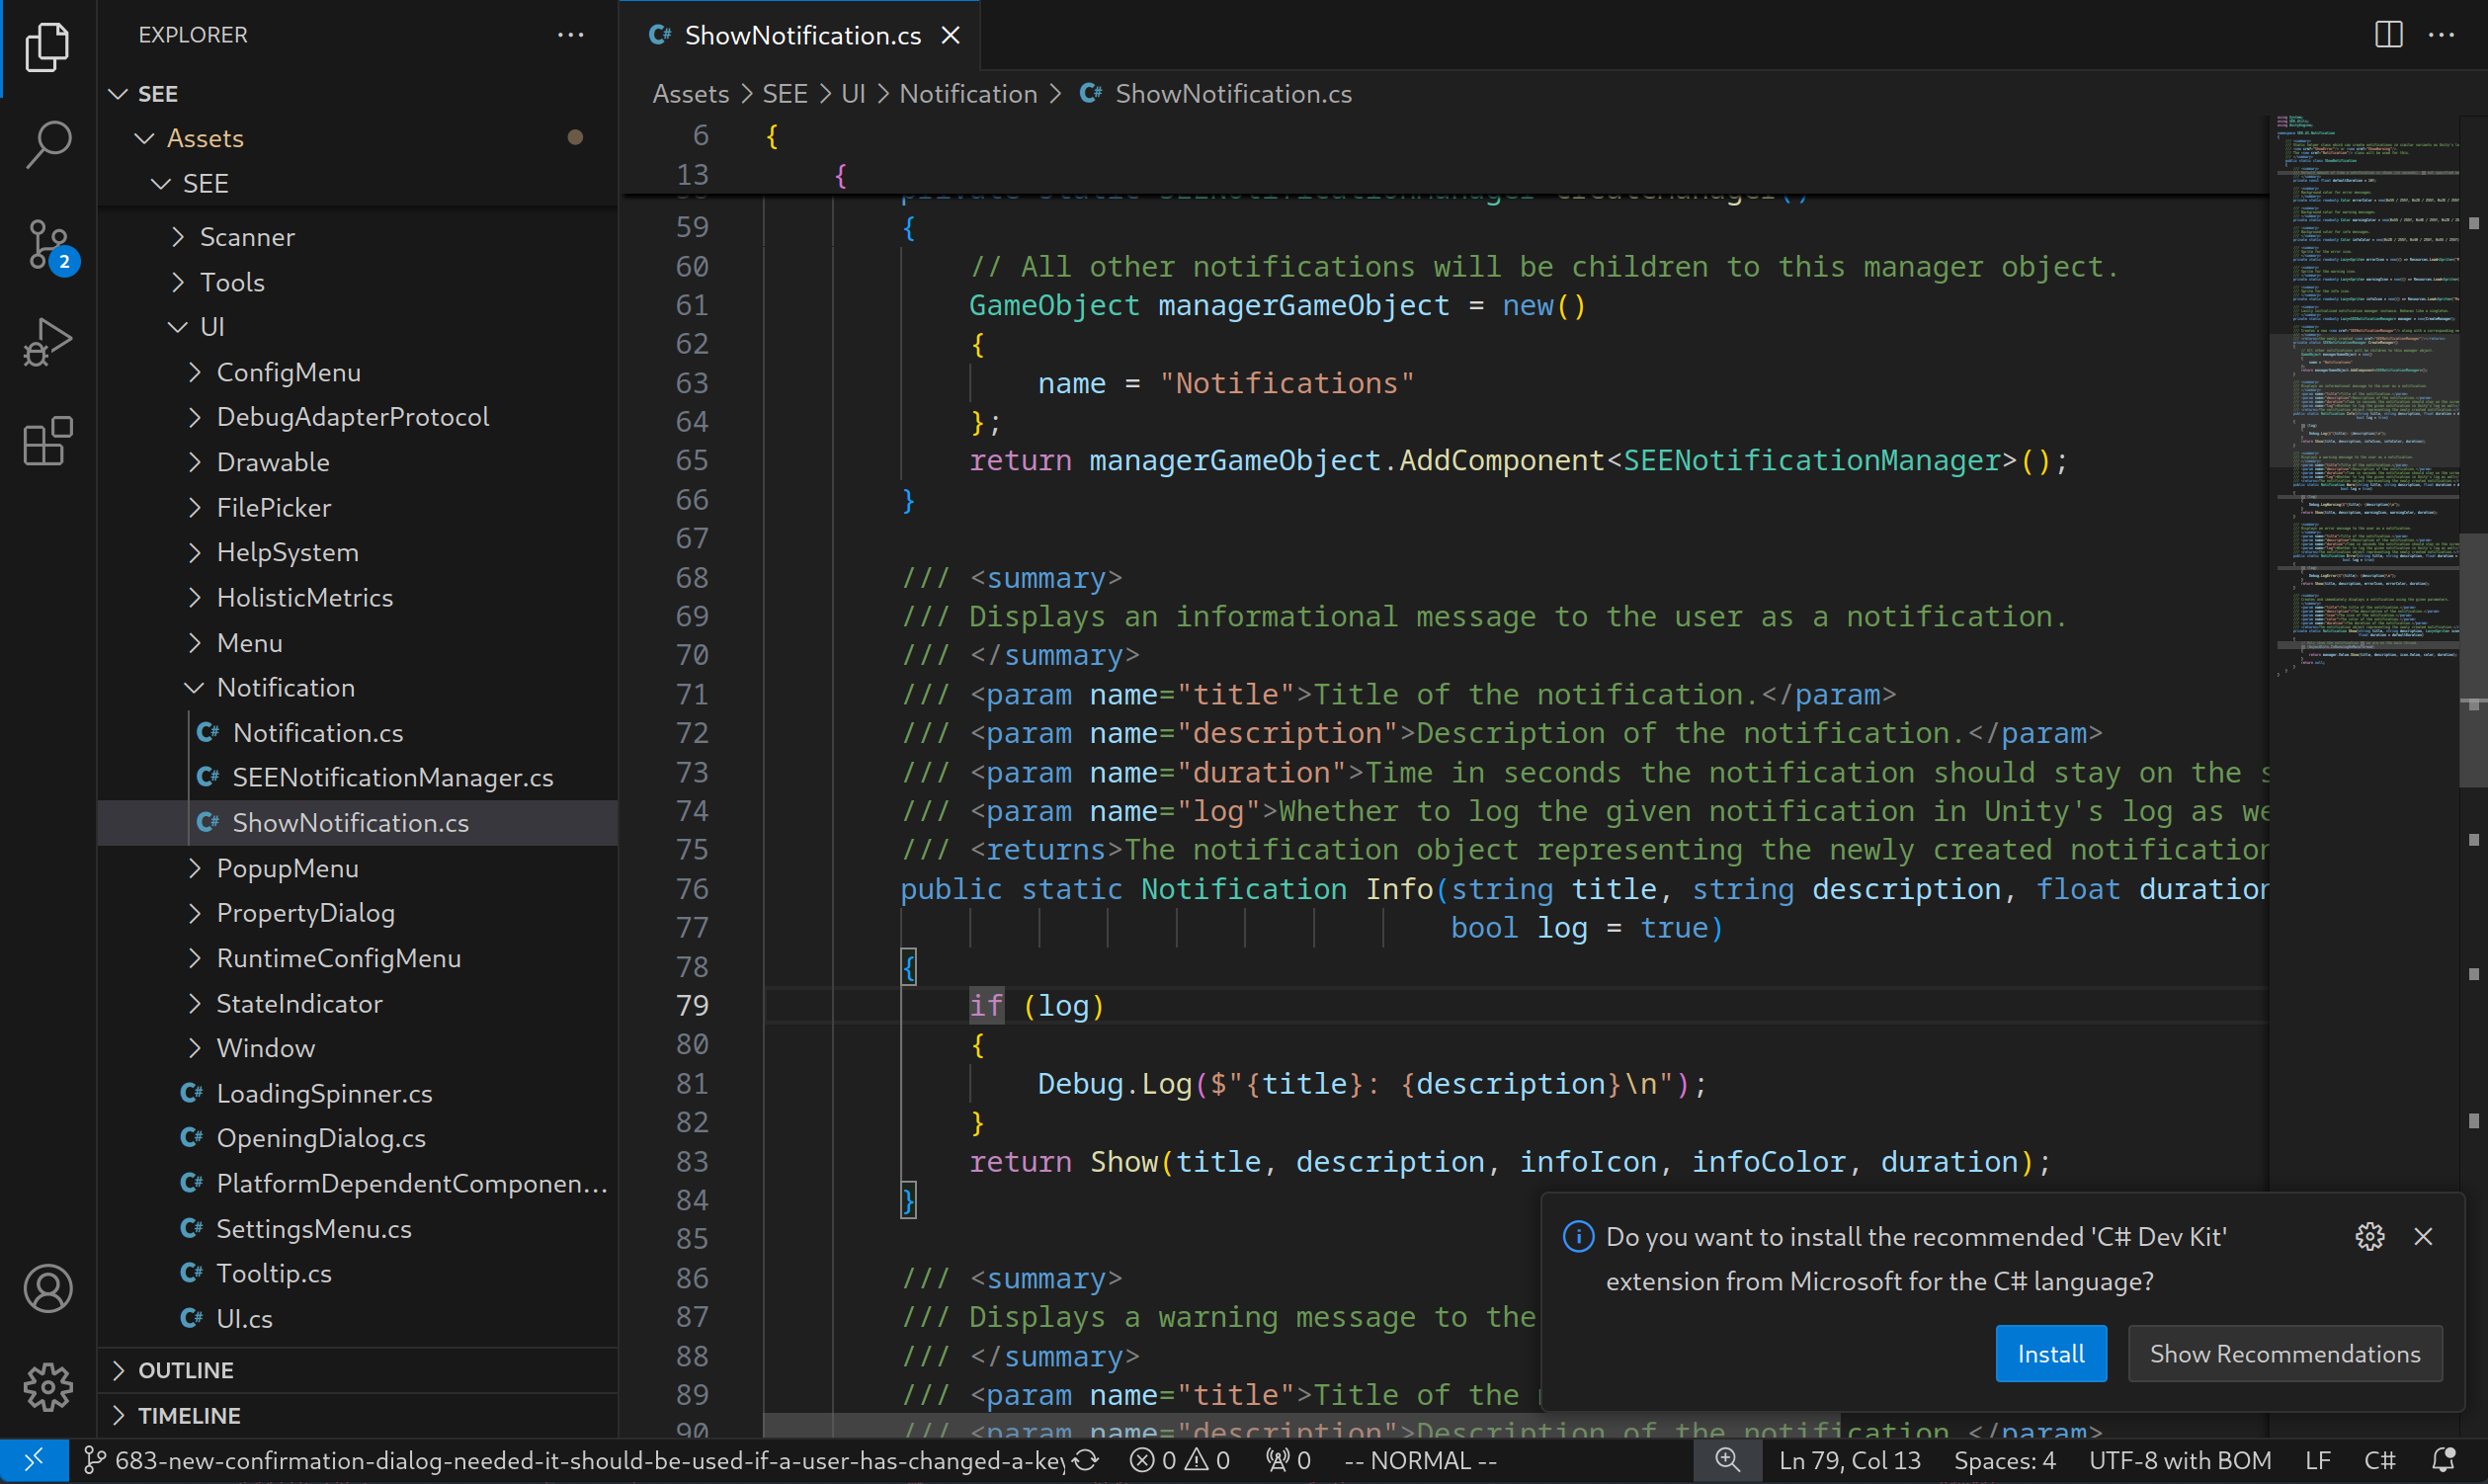
\includegraphics[width=0.95\textwidth]{VSCode}
	\end{center}
	\caption{Screenshot of the main \gls{ui} of \gls{vscode}.}\label{fig:vscode}
\end{figure}

Here, we will very briefly go over \gls{vscode} as the tool that we will compare \SEE{} against.
A screenshot of \gls{vscode} is provided in \cref{fig:vscode}.
On the left side, we can see the filesystem hierarchy of the open project, in the middle is the code itself, and on the right is a minimap as a quick overview of the current file's code.
\gls{vscode} also has an extension system in place with which \glspl{ls} and other enhancements to the editor can be easily installed---for example, we can see a notification in the bottom right prompting the user to install the C\# extension.

\begin{figure}[htbp]
	\begin{center}
		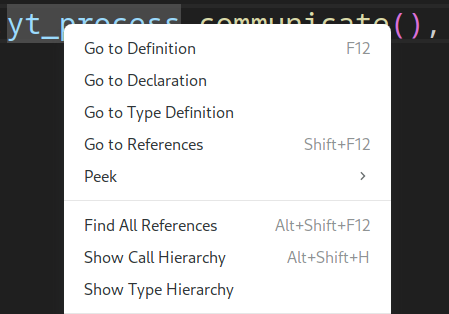
\includegraphics[width=0.5\textwidth]{VSCode-menu}
	\end{center}
	\caption{Screenshot of (the beginning of) \gls{vscode}'s context menu for code identifiers.}\label{fig:vscode_menu}
\end{figure}

It is also possible to quickly find files with the \keystroke{Ctrl} + \keystroke{P} shortcut, which pops up a menu with a live search through all filenames in the project.
The analogue in \SEE{} is the tree view which was showcased in \cref{sec:intocity}.
Also shown in that chapter was a context menu with various options to make use of the \gls{lsp} "go to location" \glspl{capability}.
\Gls{vscode} has a very similar context menu when right-clicking code identifiers, which is displayed in \cref{fig:vscode_menu}.
Additionally, \gls{vscode} users can also jump to the definition of a symbol by holding down \keystroke{Ctrl} and clicking on that symbol, the same as in \cref{sec:intowindow}.

However, a feature of \SEE{} which \emph{does not} have a clear alternative in \gls{vscode} is the ability to quickly be able to tell certain metrics, such as the number of methods in a file.
In \SEE{}, we could simply visualize that by encoding it as the size of each building, but in \gls{vscode}, participants would need to manually count each method, so to remedy this, we offer a table with such metrics.
The table is hosted on Google Spreadsheets\footnote{
	\web{https://docs.google.com/spreadsheets/d/1Z2AQDk2-XeVBB1kAtcpc18mFkPI5ZSsSz\_yOwS4pQ88}{2024-11-20} and \web{https://docs.google.com/spreadsheets/d/1erJZTwYtG-CQfZJPT-zt-chX\_VHL9jLrVfWAWZMFvEo}{2024-11-20}.
} and can be sorted by any column as well as searched.
The script with which the metrics were extracted is attached as \fxwarning*{Attach script in appendix.}{TODO}.

\subsection{Hypotheses}\label{subsec:hypotheses}

To answer \textsf{RQ2} (see \cref{sec:goals}), we would like to know whether there is any significant\footnote{
	Any mention of "significance" in this chapter refers to statistical significance.
} difference between the approaches on the dimensions of \emph{speed}, \emph{correctness}, and \emph{usability}, similar to most other studies mentioned in \cref{subsec:research}.
We will now create more concrete hypotheses for each of these dimensions.

\begin{enumerate}[label=\alph*)]
	\item \textbf{Correctness}: We call the correctness $C_S$ for tasks done in \SEE{} and $C_V$ for tasks done in \gls{vscode}.
	      This will be either a categorical variable with two possible values (\ie, correct or incorrect) or a rational number indicating the percentage of correct answers within a task.
	      \begin{itemize}
		      \item \emph{Null hypothesis} $H_{a_0}$:
		            The correctness when using \SEE{} is the same as when using \gls{vscode}: $C_S = C_V$.
		      \item \emph{Alternative hypothesis} $H_{a_1}$:
		            The correctness when using \SEE{} is different when using \gls{vscode}: $C_S \neq C_V$.
	      \end{itemize}
	\item \textbf{Speed}: We call the time it takes to finish a task $t_S$ for \SEE{} and $t_V$ for \gls{vscode}.
	      \begin{itemize}
		      \item \emph{Null hypothesis} $H_{b_0}$:
		            The time it takes to solve a task when using \SEE{} is the same as when using \gls{vscode}: $t_S = t_V$.
		      \item \emph{Alternative hypothesis} $H_{b_1}$:
		            The time it takes to solve a task when using \SEE{} is different when using \gls{vscode}: $t_S \neq t_V$.
	      \end{itemize}
\end{enumerate}

For the \textbf{usability}, we need to differentiate between the \gls{poststudy} \gls{sus} we use to evaluate the usability of the system as a whole, and the reduced 2-item \gls{posttask} \gls{asq} we use after each task (see \cref{subsec:question}).

\begin{enumerate}[resume,label=\alph*)]
	\item \textbf{\gls{sus}}:
	      We call the \gls{sus} score for \SEE{} $S_S$ and the one for \gls{vscode} $S_D$.
	      \begin{itemize}
		      \item \emph{Null hypothesis} $H_{c_0}$:
		            The \gls{sus} score for \SEE{} is the same as the \gls{sus} score for \gls{vscode}: $S_S = S_V$.
		      \item \emph{Alternative hypothesis} $H_{c_1}$:
		            The \gls{sus} score for \SEE{} is different from the \gls{sus} score for \gls{vscode}: $S_S \neq S_V$.
	      \end{itemize}
	\item \textbf{\gls{asq}}:
	      We need to once again differentiate between the two aspects that the \gls{asq} measures.
	      \begin{enumerate}[label=\roman*)]
		      \item We call the \gls{asq} score for \emph{complexity}\footnote{
			            Note that a higher score here means a lower amount of complexity.
		            } $A^c_S$ for \SEE{} and $A^c_V$ for \gls{vscode}.
		            \begin{itemize}
			            \item \emph{Null hypothesis} $H_{d_0}$:
			                  The \gls{asq} score for complexity when using \SEE{} is the same as when using \gls{vscode}: $A^c_S = A^c_V$
			            \item \emph{Alternative hypothesis} $H_{d_1}$:
			                  The \gls{asq} score for complexity when using \SEE{} is different when using \gls{vscode}: $A^c_S \neq A^c_V$
		            \end{itemize}
		      \item We call the \gls{asq} score for \emph{effort}\footnote{
			            Again, a higher score indicates less required effort.
		            } $A^e_S$ for \SEE{} and $A^e_V$ for \gls{vscode}.
		            \begin{itemize}
			            \item \emph{Null hypothesis} $H_{e_0}$:
			                  The \gls{asq} score for effort when using \SEE{} is the same as when using \gls{vscode}: $A^e_S = A^e_V$
			            \item \emph{Alternative hypothesis} $H_{e_1}$:
			                  The \gls{asq} score for effort when using \SEE{} is different when using \gls{vscode}: $A^e_S \neq A^e_V$
		            \end{itemize}
	      \end{enumerate}
\end{enumerate}

We will use a significance level of $\alpha = 0.05$ for all of our tests, though this will get halved to $0.025$ since we are using two-sided tests.

\section{Design}\label{sec:design}
Since all the hypotheses we just listed compare \SEE{} to \gls{vscode}, the general form of our study should be to have participants solve representative software engineering related tasks, with one group solving tasks in \SEE{} and the other using \gls{vscode}.
There are going to be six tasks, each taking no longer than ten minutes, which we will go over in \cref{subsec:tasks}.
To maximize the number of collected datapoints, we will have each group use both tools.
Specifically, group $\Psi$ will use \SEE{} for the first three tasks and \gls{vscode} for the last three tasks, while this will be switched around for group $\Omega$.
We will then have $\frac{n}{2}$ datapoints per tool for each task, which we can then compare against each other to test for significant differences.
This flow is illustrated in \cref{fig:taskflow}.

We have several constraints for our study.
It should be possible to partake in the study online and asynchronously (\ie, without me needing to be present) to facilitate participation and reduce the \gls{hawthorne} (though this will not completely eliminate it~\cite[\eg][]{evans2010}).
To not overexert participants and thus confound any results, the study should also be of a reasonable length---ideally, not longer than an hour (hence the number of six tasks).
Finally, we cannot assume famility with either \SEE{} or \gls{vscode}, so we need to explain the core concepts of each and verify that the participant understood them before starting the actual tasks.

Additionally, we would like to follow the "wish list" compiled by \textcite[122--124]{wettel2011}:
\newcommand{\cyes}{\textcolor{ForestGreen}{\textbf{[\ding{51}]}}}
\newcommand{\chmm}{\textcolor{BurntOrange}{\textbf{[\textit{?}]}}}
\newcommand{\cno}{\textcolor{Maroon}{\textbf{[\ding{55}]}}}
\begin{enumerate}
	\item \textbf{\enquote{Avoid comparing using a technique against not using it.}}
	      We are comparing \gls{vscode} against \SEE{}. \cyes
	\item \textbf{\enquote{Involve participants from industry.}}
	      Roughly half of our participants have reported working on bigger software projects (either within a company or as open-source contributions) for at least 3 years. \cyes
	\item \textbf{\enquote{Provide a not-so-short tutorial of the experimental tool to the participants.}}
	      We do give a tutorial of each tool to participants, but it only covers the essentials required for the tasks (since we do not want to drag out the participation longer than necessary.) \chmm
	\item \textbf{\enquote{Avoid, whenever possible, to give the tutorial right before the test.}}
	      Unfortunately, we cannot really avoid this.
	      Wettel suggests performing the training a few days before the study, but this is intractable for this study. \cno
	\item \textbf{\enquote{Use the tutorial to cover both the research behind the approach and the implementation.}}
	      The motivation here would be to provide another incentive to participate out of interest in furthering the research.
	      We have left out the research both to keep the participation short and to avoid biasing participants (\eg, by claiming beforehand that developers find \glspl{city} much nicer to use than \glspl{ide}). \cno
	\item \textbf{\enquote{Find a set of relevant tasks.}}
	      Our tasks are representative of real-world activities (see \cref{subsec:tasks}), but some may turn out to have been too easy, as we will see in the analysis in \cref{subsec:correct}. \chmm
	\item \textbf{\enquote{Choose real object systems that are relevant for the tasks.}}
	      We have chosen \emph{SpotBugs} (3.5k GitHub stars, $\approx$ 216 k\gls{loc}) and \emph{JabRef} (3.6k GitHub stars, $\approx$ 179 k\gls{loc}). \cyes
	\item \textbf{\enquote{Include more than one subject system in the [experiment].}}
	      See first item. \cyes
	\item \textbf{\enquote{Provide the same data to all participants.}}
	      The tasks for both participants (and accompanying data) are identical, and \gls{vscode} participants get access to a table of metrics so that the same data is present. \cyes
	\item \textbf{\enquote{Limit the amount of time allowed for solving each task.}}
	      Integrating a limit like this into the tool we used for the questionnaire would have proved difficult, but the tasks were comparatively simple and participants were aware that their completion time was measured, so we should hopefully have avoided the effects Wettel references here. \chmm
	\item \textbf{\enquote{Provide all the details needed to make the experiment replicable.}}
	      I have included (pseudonymized) participation data, the full definition of the questionnaire, and the analysis script which performed data cleanup and statistical tests. \cyes
	      \fxwarning{Link to appendix here.}
	\item \textbf{\enquote{Report results on individual tasks.}}
	      We are going over each task individually when reporting results in \cref{sec:results}. \cyes
	\item \textbf{\enquote{Take into account the possible wide range of experience level of the participants.}}
	      We are taking a detailed look at the effects of experience in \cref{subsec:experience}. \cyes
\end{enumerate}

In total, we were able to fulfill 7/13 items on the wish list, with 3/13 being questionably/partially fulfilled and 2/12 not being implemented, with the reasoning for the latter two being that it would otherwise lengthen the participation time and may strain participants.

\subsection{Questionnaires}\label{subsec:question}
There are three questionnaires that we are going to use for this study:
A demographic questionnaire, a \gls{posttask} questionnaire and a \gls{poststudy} questionnaire, where we will use the latter two to get an estimation on usability.
We are also going to take a look at \emph{KoboToolbox}, the tool we are using to asynchronously conduct our survey.
An important general consideration is that we will offer our study in both English and German, so any questionnaire we choose (which is usually given in English) needs to have a validated German translation to make results comparable.
This section partially mirrors similar considerations from my bachelor's thesis, which the interested reader can peruse for more details~\cite{galperin2021}.
For a comprehensive overview and evaluation of other \gls{poststudy} and \gls{posttask} questionnaires covered neither here nor in my bachelor's thesis, see the review by \textcite{hodrien2021}.

\paragraph{Demographics}
We ask each participant various demographic questions to (among other reasons) address the threat to validity of selection bias:
While participants are randomly assigned into groups $\Psi$ and $\Omega$, it is of course possible due to our moderate sample size of $n = \participants$ that there is a significant difference in any independent variable.
A difference like this would then matter if it acts as a confounder for one of the dependent variables---for example, age or experience can have a sizable impact on \gls{sus} scores~\cites[585]{bangor2008}{mclellan2012}.

To catch this, we ask for some properties that could be relevant, namely
gender, age, programming experience, professional programming experience, knowledge of \SEE{}, knowledge of \gls{vscode}, knowledge of JabRef, knowledge of SpotBugs, and experience with 3D video games.
We ask the last question since \SEE{} uses some typical video game paradigms for its controls, so a familiarity with such controls may make \SEE{} more intuitive to use for those people.
Additionally, we ask if the participant has ever used \glspl{ide} before, and if they are able to use the Java programming language.
If the answer to either of those questions is "no," we display a warning telling the participant that this study is not intended for them and may be too difficult (as both JabRef and SpotBugs are Java projects).
We will later filter participations with "no" answers out of our dataset to avoid these problems.

\paragraph{\Gls{posttask}: \gls{asq}}
This questionnaire will be filled out by the participant after each task---since there are six tasks, this will be six times total.
For this reason, we should keep this one short, that is, no more than three questions long, which eliminates questionnaires such as NASA's \gls{tlx}.
There are also the rather unconventional \gls{ume} (which we exclude since it often confuses its users~\cite[1607--1608]{sauro2009b}) or \gls{smeq} (which we exclude because this would be hard to implement in our online questionnaire).
Instead, we choose the \emph{\glsentrylong{asq}}, which consists of three statements for which users give answers on a \gls{likert}:
\begin{enumerate}
	\item \enquote{Overall, I am satisfied with the ease of completing the tasks in this scenario.}
	\item \enquote{Overall, I am satisfied with the amount of time it took to complete the tasks in this scenario.}
	\item \enquote{Overall, I am satisfied with the support information (on-line help, messages, documentation) when completing the tasks.}
\end{enumerate}

We exclude the last question since we neither offer nor want to measure usage of such support information.
However, the rest is ideal for our case:
The \gls{asq} is short, easy to understand, and distinguishes between cognitive and temporal ease---we will call "cognitive ease" \emph{complexity} and "temporal ease" \emph{effort} (as in \cref{subsec:hypotheses}).
The translation by \textcite[32]{roegele2020} will serve as the German version.

\paragraph{\Gls{poststudy}: \gls{sus}}
We will present this questionnaire once after the \SEE{} section and once after the \gls{vscode} section, and will use it to collect a general usability score of each system.
Since the questionnaire is filled out twice, we set an upper limit of twenty questions.
This eliminates both the \gls{sumi} and \gls{quis} from consideration.
Because we need a validated German translation, we can also strike out the English-only \gls{pssuq} as an option.

This leaves the \emph{\glsentrylong{sus}} as a fitting option:
It has a validated German translation~\cite{reinhardt2015}, is the most used \gls{poststudy} questionnaire for this purpose~\cites[1615]{sauro2009}[577]{lewis2018}, and is very well-suited for comparing two systems or interfaces~\cites[195]{peres2013}[590--591]{bangor2008}.
It consists of ten \gls{likert} questions which alternate between positive and negative aspects of the system and returns a score between 0 and 100, representing the system's usability~\cite{brooke1996}.
Existing measured \gls{sus} scores for \SEE{} are given in \cref{fig:seesus}.

\paragraph{KoboToolbox}
The tool with which we manage the survey needs to handle our requirements for it to be feasible to conduct it asynchronously.
Specifically, we need to:
\begin{itemize}
	\item reliably measure the time each task takes to solve,
	\item provide both an English and a German version of the questionnaire,
	\item ask questions with numerical, text-based, selection, and \gls{likert}-based input, and
	\item conditionally show fields or bar the user from continuing (\eg, until the tutorial question is answered correctly) depending on existing input.
\end{itemize}
Among the tools that can handle this for free, \textit{KoboToolbox}\footnote{
	\web{https://www.kobotoolbox.org/}{2024-11-23}
} seems like the most mature, robust option.
It accepts form based on the \gls{xlsform} specification, which makes forms (relatively) easy to create with a spreadsheet editor.

Before each task, we tell the user beforehand that their time will be measured as soon as they advance to the next page.
Then, we keep a timestamp for each editable field in the task, including a checkbox the user can check to indicate they have finished the task.
Using the set of those timestamps $T$ and the timestamp $t_0$ of when they started the task, the time for the task can then be calculated as $\max T - t_0$.
This also ensures we catch "cheating" in the form of participants editing fields after they have indicated they are finished with the task.
The survey in \gls{xlsform} is linked in \fxwarning*{Link to questionnaire in appendix}{TODO}, and a screenshot of the starting page is shown in \cref{fig:kobo}.

\begin{figure}
	\begin{center}
		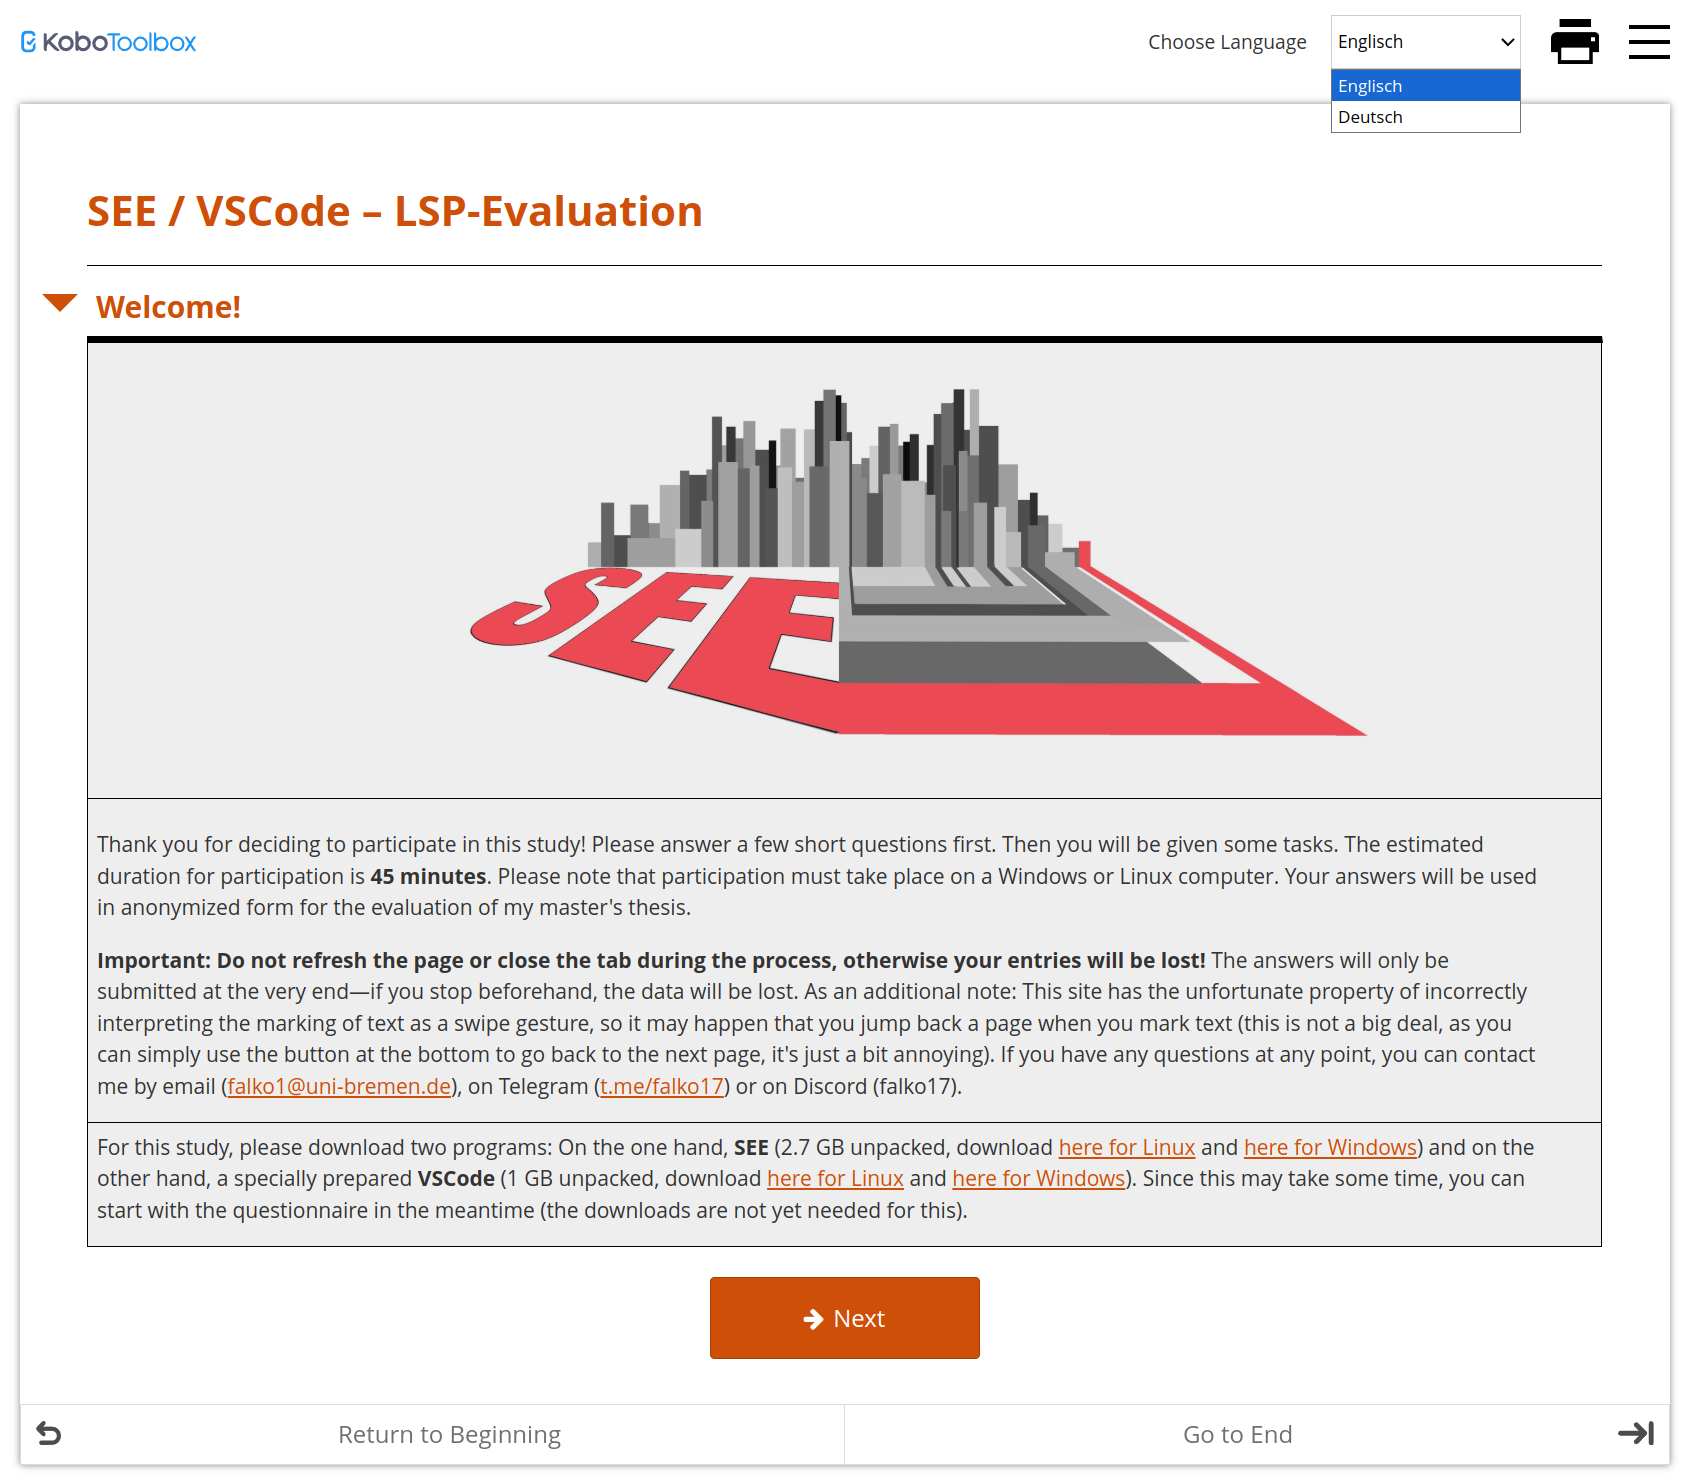
\includegraphics[width=0.95\textwidth]{Kobo.png}
	\end{center}
	\caption{Starting page of the survey built with KoboToolbox.}\label{fig:kobo}
\end{figure}


To equally partition participants into two groups, we create two versions of the survey, one for group $\Psi$ and one for group $\Omega$.
We then access KoboToolbox's REST API to redirect the participants to version $\Psi$ or $\Omega$---the algorithm we are using is given in \cref{alg:redirect}, or can alternatively be seen in \fxwarning*{Link to script in appendix}{TODO}.
Inviting others to participate then becomes as simple as passing the link to the redirection script around\footnote{
	\url{https://falko.de/master-evaluation}, but this link may not stay up forever.
}.

\begin{algorithm}
	\tikzexternaldisable
	\caption{How participants are redirected to the two versions of the survey.}\label{alg:redirect}
	\begin{algorithmic}[1]
		\small
		\Require{Participant ID $p$ retrieved from cookie in request, or $\varnothing$ if it does not exist.}
		\Ensure{Tuple consisting of the participation ID to be set as a cookie and a survey link.}
		\LComment{Global state: $P$ is an initially empty mapping from IDs to links, $i$ is initially zero.}
		\If{$p \notin P$}
		\If{$p = \varnothing$}
		\State $p = \Call{NewRandomID}{\null}$
		\EndIf
		\State $n_{\Psi}, n_{\Omega} \gets \Call{GetKoboParticipations}{\null}$
		\If{$n_{\Psi} = \varnothing \lor n_{\Omega} = \varnothing$}
		\Comment{API request failed, so just alternate using index $i$.}
		\If{$i = 0$}
		\State $P(p) \gets \Psi$
		\Else
		\State $P(p) \gets \Omega$
		\EndIf
		\State $i \gets (i + 1) \bmod 2$
		\ElsIf{$n_{\Psi} \leq n_{\Omega}$}
		\State $P(p) \gets \Psi$
		\Else
		\State $P(p) \gets \Omega$
		\EndIf
		\EndIf
		\State \Return $(p, P(p))$
	\end{algorithmic}
	\tikzexternalenable
\end{algorithm}

\subsection{Tasks}\label{subsec:tasks}
As explained in \cref{sec:plan}, we cannot feasibly evaluate most implemented \gls{lsp} \glspl{capability} except for the generation of the \gls{city} itself.
This means we are actually comparing a \gls{city} against an \gls{ide}, with \gls{lsp} only playing the role of providing us with those \glspl{city}, for which there are a number of existing experiments that we went over in \cref{subsec:research}.
Thus, we should base our own study design on the existing literature established in that section.
Specifically, out of the similar studies collected in \cref{tab:compresults}, the study by \textcites{wettel2011} (replicated by \textcite{romano2019}) seems most fitting for us:
It compares a Desktop \gls{city} implementation against a traditional \gls{ide} along with providing \gls{csv} metrics to make the comparison fair.
In addition, it provides a great number of details, including detailed task definitions, and a wish list which we went over at the beginning of \cref{sec:design}.

Wettel uses two kinds of tasks~\cite[128--130]{wettel2011}:
Those concerened with program comprehension and those concerned with design quality assessment.
Of these, the latter requires deeper software engineering knowledge that may not be present in all participants, since a large proportion of them are still going to be students.
Thus, we will focus on tasks from the first group:
\begin{enumerate}
	\item \enquote{Locate all the unit test classes of the system and identify the convention (or lack of convention) used by the system’s developers to organize the unit tests.}
	      \begin{description}
		      \item[\follows{}] This task seems like a nice fit to realistically evaluate usage of both tools, so we include it.
		            We will call it \textbf{task $\bm{B}$}.
	      \end{description}
	\item \enquote{Look for the term $T$ in the names of the classes and their attributes and methods, and describe the spread of these classes in the system.}
	      \begin{description}
		      \item[\follows{}] The concept of "spread" would take time to properly introduce and may be misunderstood by some participants, so we exclude this task.
	      \end{description}
	\item \enquote{Evaluate the change impact of class $C$ defined in package $P$, by considering its caller classes. The assessment is done in terms of both intensity and dispersion.}
	      \begin{description}
		      \item[\follows{}] This seems like a complex task that takes time both to properly understand it and then also to execute it, so we exclude it.
	      \end{description}
	\item \enquote{Find the three classes with the highest \gls{nom} in the system.}
	      \begin{description}
		      \item[\follows{}] This task also seems simple to understand and probably will not take too long, so we include it.
		            We will call it \textbf{task $\bm{A}$}.
	      \end{description}
\end{enumerate}

Note, however, that none of the tasks we selected above test any edge-related behavior, so we will add one task of our own.
This \textbf{task $\bm{C}$} will be to \enquote{find the \gls{base} for class $c$ in the system.}
Its drawback is that it requires a short explanation of \glspl{base} before the task, but its upsides are that it is both a realistic task and additionally forces participants to have more than a cursory interaction with the edges (specifically, the \tt{Extend} edges\footnote{
	We should also note that the \glspl{city} for this study \emph{only} contain \tt{Extend} edges---otherwise, there are too many edges for \SEE{} to handle in a performant manner.
}) without having any unfair disadvantage in \gls{vscode}, where participants can navigate up the inheritance tree by repeatedly \keystroke{Ctrl}-clicking on the superclass.

Now we only need to choose a fitting $c$ for both JabRef and SpotBugs, our two object systems.
To make sure the task is not too easy, we choose the class which is deepest in the inheritance tree for both system.
For JabRef, this is \tt{GenderEditorViewModel} (five levels deep), while for SpotBugs, this is \tt{OptionalReturnNull} (seven levels deep).
This way, we can also evaluate the transitive edge animations we added in \fxwarning*{Where?}{some section}.

We should also mention that, for task $B$, like Wettel, we give multiple choice options for the various kinds of conventions along with brief descriptions to make sure they are understood correctly.
If one of the options is then chosen (\eg, \enquote{Centralized}), users have to give follow-up information (\eg, \enquote{What is the full name of the root package for test classes?}) to make sure the correct answer was not just guessed.
A full visual overview of our study along with its tasks is given in \cref{fig:taskflow}.

\begin{figure}
	\begin{center}
		\begin{tikzpicture}[
			box/.style={draw, rounded corners, text width=6cm, align=center, minimum height=2cm},
			scalebox/.style={draw, rounded corners, text width=4.5cm, align=center, minimum height=1cm},
			heading/.style={font=\Large\bfseries\boldmath},
			nextarrow/.style={draw=Maroon, line width=0.5mm,-{Latex[length=3mm]}}
			]

			\newcommand{\taskbox}[5][]{\node[box,#1] (#2) at (#3) {{\large\bfseries\boldmath \underline{#4}}\\\vspace{1.5mm}\small#5}}

			% Left title box.
			\node[draw, thick, minimum width=7cm, minimum height=14.5cm] (left) at (0,0) {};
			\node[heading,align=center] at (0,6.4) {Group $\Psi$: SEE\\Group $\Omega$: VSCode};

			% Boxes for tasks to the left.
			\node[scalebox] (D) at (0, 4.4) {\itshape\color{Gray!50!Black}Demographics};
			\taskbox{A1}{$(D) + (0, -2.3)$}{Task $A_1$}{Find the three classes with the highest number of methods in SpotBugs.};
			\taskbox{B1}{$(A1) + (0, -3)$}{Task $B_1$}{Identify the convention used by the developers to organize the unit tests in SpotBugs.};
			\taskbox{C1}{$(B1) + (0, -3)$}{Task $C_1$}{Find the base type for class \texttt{OptionalReturnNull} in SpotBugs.};
			\node[scalebox] (S1) at ($(C1) + (0,-2.3)$) {\itshape\large\glsentrylong{sus}};

			% Right title box.
			\node[draw, thick, minimum width=7cm, minimum height=14.5cm] (right) at (8,0) {};
			\node[heading,align=center] at (8,6.4) {Group $\Psi$: VSCode\\Group $\Omega$: SEE};

			% Boxes for tasks to the right.
			\taskbox[anchor=north]{A2}{8, |- D.north}{Task $A_2$}{Find the three classes with the highest number of methods in JabRef.};
			\taskbox{B2}{$(A2) + (0, -3)$}{Task $B_2$}{Identify the convention used by the developers to organize the unit tests in JabRef.};
			\taskbox{C2}{$(B2) + (0, -3)$}{Task $C_2$}{Find the base type for class \texttt{GenderEditorViewModel} in JabRef.};
			\node[scalebox] (S2) at ($(C2) + (0, -2.3)$) {\itshape\large\glsentrylong{sus}};
			\node[scalebox] (C) at (S2 |-, |- S1) {\itshape\color{Gray!50!Black}Final comments};

			% Lines below heading at top
			\node[inner sep=0pt] at ($(left.north east)!.5!(left.north west) + (0,-1.8)$) {\pgfornament[width=7cm]{88}} ;
			\node[inner sep=0pt] at ($(right.north east)!.5!(right.north west) + (0,-1.8)$) {\pgfornament[width=7cm]{88}} ;

			% And the arrows.
			\draw[nextarrow] (D) -- (A1);
			\draw[nextarrow] (A1) -- (B1);
			\draw[nextarrow] (B1) -- (C1);
			\draw[nextarrow] (C1) -- (S1);
			\draw[nextarrow] (A2) -- (B2);
			\draw[nextarrow] (B2) -- (C2);
			\draw[nextarrow] (C2) -- (S2);
			\draw[nextarrow] (S2) -- (C);
			\draw[nextarrow] (S1.east) to[out=0,in=180] (A2.west);
		\end{tikzpicture}
	\end{center}
	\caption{Flow of the tasks the participants worked on.
		$A^c$ and $A^e$ were gathered after each task.
	}\label{fig:taskflow}
\end{figure}


\section{Results}\label{sec:results}
In this section, we can finally report on the results of the study.
We will first go over the course of how the study was conducted before taking a look at the results themselves.
For the latter, we start by analyzing the answers to the demographics questionnaire, and then go on to interpret the dependent variables relevant to our hypotheses, namely, correctness, time, and usability, in that order.
We will then also investigate the role of experience (and some other independent variables) and the influence it had on how tasks were handled.
Finally, we handle the various comments that were left during the study.

As mentioned before, we use a significance level of $\alpha = 0.05$.
We can neither assume normal distributions for our data, nor is it always interval-scaled, so we choose the \gls{mwu} to determine statistically significant differences between either our two groups $\Psi$ and $\Omega$ or between the two tools \SEE{} and \gls{vscode}.
To help the reader quickly identify important results, we put a star ($\bigstar$) in the heading of a paragraph to indicate that it lead to the rejection of a null hypothesis.

% \Psi and \varomega

% TODO: Maybe mention alpha error stuff here already if relevant?
%       As well as alpha=0.05. Don't call it alpha due to confusion with alphabeta. 
%       And some stats stuff here maybe, such as why MWU.

\subsection{Study Procedure}
Before we started with the actual study, we did a small-scale pilot study with two participants, one of them being this thesis's first reviewer Prof.\ Dr.\ Rainer Koschke.
Through their valuable feedback, I was able to see some issues I had not noticed myself before starting the study, such as a few bugs in \SEE{}, confusion regarding the term \gls{base}, and errors unpacking the prepared compressed builds of \SEE{} and \gls{vscode}\footnote{
	As a sidenote, using prepared builds also prevents any potential problems.
	For example, some pre-installed plugins of \gls{vscode} might otherwise interfere with our study.
} when using Windows.
I fixed the bugs in \SEE{}, added a tutorial for the \glspl{base} (along with a comprehension question), and added detailed instructions on how to correctly unpack the builds.
There luckily were no other major issues in the actual study after these problems noticed in the pilot study have been ironed out.

There have been \participants participants in total, though we had to exclude one participant from most analyses because he indicated he had no knowledge of Java.
Participants were gained via convenience sampling, that is, I asked fellow students, colleague developers from Axivion, and other acquaintances who had software engineering experience to participate.

\fxnote{In Appendix, give answer key.}

\subsection{Demographics}

First, we want to take a quick look at the demographics of our study.
We also take this opportunity to find any significant differences between the two groups $\Psi$ and $\Omega$, to make sure any results in the dependent variables later on are not just due to such differences.
For this purpose, we define null hypotheses of the form \enquote{Variable $X$ is not different between groups $\Psi$ and $\Omega$}, which we check with a two-sided \gls{mwu}, as we cannot assume normal distributions.
This also allows us to compare merely ordinal data.

All answers\footnote{
	The question "Do you know SpotBugs?" has also been excluded from the bar charts, as only one participant answered "I've heard of it", with all others answering "no".
} to the demographic questions can be viewed as bar charts in \cref{fig:demobars}.
Two exceptions are the non-categorical variables, namely age and the total time it took participants to finish the study, which we are going to go over first.
We have also excluded the question "Have you ever used the program SpotBugs?", as there was only one participant answering "Heard of it", with all others answering "No."


\paragraph{Age}
We have a median age of $\widetilde{A} = 29$ and an average age of $\overline{A} = 28.55$ in our sample, suggesting few outliers, which can be confirmed by looking at the violin plots in \cref{fig:dat_age}.
The \gls{mwu} also confirms no differences between the groups ($U = 40.5, p \approx 0.4947$).

\begin{figure}
	\begin{center}
		\violinab{age}{ylabel=Age}{15}{45}{3.1029}{1}
	\end{center}
	\caption{Distribution of age between the two groups.}\label{fig:dat_age}
\end{figure}

\paragraph{Total Time}
The median time it took to complete the whole study was an hour and six minutes, which means we slightly overshot our initial aim of an hour to complete the study.
In addition, the average being at roughly one and a half hours points to there being some significant outliers:
In fact, some participations were longer than 2 hours, with one participant in the $\Omega$ group even taking almost five hours---however, as no participation took longer than twenty minutes (see \cref{subsec:time}), we can conclude that this must be due to breaks in between tasks rather than the participation being actually that long.
The same likely applies to the other participations around the three hour range.
The various times are visualized in \cref{fig:dat_totaltime}, where it also becomes apparent that the two groups had similar total times, which a \gls{mwu} confirms for us ($U = 63, p \approx 0.34470$).

\begin{figure}
	\begin{center}
		\violinab{total-time}{ylabel={Time (in hours)}}{0}{5}{0.1171}{0.106}
	\end{center}
	\caption{Total duration of time in which each participant finished the study.\\
		May include time in which participants took breaks.}\label{fig:dat_totaltime}
\end{figure}

\begin{figure}
	\begin{subfigure}[T]{0.55\textwidth}
		\caption{"What is your highest school or university degree?"\label{fig:degreebar}}
		\barplot{alphabeta-degree}{Fachabitur,Abitur,Bachelor's degree,Master's degree,Doctoral degree}{width=\textwidth, enlarge x limits={0.4}}
	\end{subfigure}\hfill
	\begin{subfigure}[T]{0.45\textwidth}
		\caption{"How long have you been programming?"\label{fig:programmingbar}}
		\barplot{alphabeta-programming}{Less than 3 years, 3–9 years, 10–19 years}{width=\textwidth, ylabel={},enlarge x limits={0.7}}
	\end{subfigure}\\
	\begin{subfigure}[T]{0.55\textwidth}
		\caption{"Do you know \gls{see}?"\label{fig:knowseebar}}
		\barplot{alphabeta-knowsee}{No, Heard of it, Used it before, Developed parts of it}{width=\textwidth, enlarge x limits={0.5}}
	\end{subfigure}\hfill
	\begin{subfigure}[T]{0.45\textwidth}
		\caption{"Do you know \gls{vscode}?"\label{fig:knowvsbar}}
		\barplot{alphabeta-knowvs}{No, Heard of it, Used it before, Is my main IDE}{width=\textwidth, ylabel={}, enlarge x limits={1}}
	\end{subfigure}\\
	\begin{subfigure}[T]{0.55\textwidth}
		\caption{"Have you ever used the program JabRef?"\label{fig:knowjabrefbar}}
		\barplot{alphabeta-knowjabref}{No, Heard of it, Used it before, Developed parts of it}{width=\textwidth, enlarge x limits={0.5}}
	\end{subfigure}\hfill
	\begin{subfigure}[T]{0.45\textwidth}
		\caption{"Do you play 3D video games for desktops?"\label{fig:knowgamebar}}
		\barplot{alphabeta-knowgame}{I never played, I barely play, I play a lot}{width=\textwidth, ylabel={}, enlarge x limits={0.7}}
	\end{subfigure}
	\caption{Number of respective answers to various demographic questions.\\
		Group \textcolor{Maroon}{$\Psi$ is in red}, and group \textcolor{Gray!50!black}{$\Omega$ is in gray}.}\label{fig:demobars}
\end{figure}

\paragraph{Degree}
Most participants had a Bachelor's degree (this is also the median), with some Abitur degrees, Master's degrees, and one person with a doctoral degree (see \cref{fig:degreebar}).
The \gls{mwu} reveals no significant differences between $\Psi$ and $\Omega$ ($U = 57.5, p \approx 0.5693$).

\paragraph{$\bigstar$ Programming Experience}
Both the median and modal programming experience is 3--9 years.
However, we can see that the only people with 10--19 years of experience are in group $\Psi$, and the \gls{mwu} indeed confirms a significant difference here ($U = 77, p \approx 0.0214$).
It is unclear how this could have happened except coincidentally, as participants were always alternatingly assigned to either group $\Psi$ and $\Omega$.
Nonetheless, we need to keep this difference in mind when moving on to the analysis of dependent variables.

\paragraph{$\bigstar$ Experience on Bigger Software Projects}

\begin{wrapfigure}{L}{0.5\textwidth}
	\centering
	\barplot{alphabeta-opensource}{Not yet, Less than 3 years, 3–9 years}{width=0.5\textwidth,ymax=10,height=5.2cm,enlarge x limits={0.6}}
	\caption{"How long have you been programming on bigger software projects (\eg, within a company, or open-source projects)?"}\label{fig:opensourcebar}
\end{wrapfigure}

We also asked participants for experience with larger software projects, such as within companies or on open-source projects.
Here, all but one participant have been working on bigger software projects, but the split between the "Less than 3 years" and "3--9 years" categories are inverted between groups $\Psi$ and $\Omega$, which can also be seen in \cref{fig:opensourcebar}.
The \gls{mwu} again confirms a significant difference ($U = 80.5, p \approx 0.0105$).

\paragraph{Experience with \SEE{}}
The clear majority of participants (eleven people) have developed on \SEE{} before, as can be seen in \cref{fig:knowseebar}, which can be attributed to the fact that one major group of people I asked to participate are the students who are working on \SEE{} in a professional or academic capacity.
We can also see a qualitative difference between the two groups:
Group $\Omega$ contains the only people who have answered "No", while group $\Psi$ contains the only people who have answered "I heard of it" and "I used it before".
However, this difference is not significant ($U = 42.5, p \approx 0.5598$).

\paragraph{Experience with \gls{vscode}}
Every single participant has used \gls{vscode} before, with six people even using it as their main \gls{ide}.
We can assume that most participants thus have more experience with \gls{vscode} than \SEE{}, which may bias our results somewhat---we try to investigate this further in \cref{subsec:experience,sec:threats}.
\Cref{fig:knowvsbar} shows the groups to be quite similar, and indeed, there is no significant difference here ($U = 55, p \approx 0.6809$).

\paragraph{Experience with JabRef}
Most participants in either group have not heard of JabRef before, but in contrast to SpotBugs, some have actually used the bibliography manager before, with one participant in group $\Psi$ even having developed parts of it (see \cref{fig:knowjabrefbar}).
Again, there is no significant difference between the two groups ($U = 58, p \approx 0.5041$).

\paragraph{Experience with Video Games}
A clear majority of sixteen participants reported that they play a lot of video games (as can be seen in \cref{fig:knowgamebar}), with only two responding that they barely play and one stating that they never played video games before.
Here as well there is no significant difference we need to be aware of ($U = 46, p \approx 0.6701$).

In summary, the only significant differences between the two groups that could cause problems in our analysis are the programming experience in general and the programming experience for bigger projects, both of which indicate significant differences insofar that group $\Psi$ apparently contains more experienced programmers.
We will investigate the effects of this in more detail in \cref{subsec:experience}.

% % TODO: ordinal data
%
% \violinsv{a1-time}{Time (Minutes)}{0}{20}
% \violinsv{a2-time}{Time (Minutes)}{0}{20}
% \violinsv{a3-time}{Time (Minutes)}{0}{10}
% \violinsv{a4-time}{Time (Minutes)}{0}{10}
% \violinsv{a5-time}{Time (Minutes)}{0}{20}
% \violinsv{a6-time}{Time (Minutes)}{0}{10}
%
% \violinsus{}

% \begin{tikzpicture}
% 	\violinsetoptions[data points,scaled,averages]{
% 		xmin=0,xmax=3,
% 		ymin=50,ymax=100,
% 		xlabel={Sys},
% 		xlabel style={
% 				yshift={-0.5cm},
% 			},
% 		ylabel={SUS},
% 		ymajorgrids=true,
% 		set layers
% 	}
%
% 	\violinplot[%
% 		index=sus,%
% 		col sep=tab,%
% 		color=Maroon,%
% 		dataset size=3pt,%
% 		average size=4pt,%
% 		average opacity=0.8,%
% 		average color=black,%
% 		dataset opacity=0.8,%
% 		dataset jitter=0.1,%
% 		relative position=1,%
% 		average fill opacity=0.5,%
% 		average fill=ForestGreen,%
% 		average mark=otimes*,%
% 		dataset color=black,%
% 		dataset fill=black,%
% 		dataset fill opacity=0.5,%
% 		label={SEE}
% 	]{analysis/dat/sus.dat}
% \end{tikzpicture}

\subsection{Correctness}\label{subsec:correct}
To evaluate the correctness of the various answers, I wrote a script which showed me each answer and prompted me to say whether this answer was correct or incorrect, while I used the previously created answer key (see {TODO}) as a base.
This allowed me to catch misspellings or unusual formats\footnote{For example, some participants also entered the \gls{nom} along with the class name for task $A$.} and still mark the answers as correct.
The results of which answers I marked as correct are attached as {TODO}, while the script used to do so is part of the general analysis script in {TODO}.
\fxwarning{Attach and link answer key, correctness answers, script in appendix}

It does not make much sense to use \glspl{violin} here, as there are in most cases only two possible values here:
The participants were either correct or incorrect in their answer to the task.
Even for task $A$, where three answers had to be given, we only have at most three possible values in practice.
For this reason, we are using bar graphs again, which are collected in \cref{fig:correctness} along with the respective results of the \gls{mwu}.

\begin{figure}
	\begin{subfigure}[T]{0.5\textwidth}
		\caption{Achieved correctness for task $A_1$.\\
			($U = 46, p \approx 0.939$)
			\label{fig:a1c}}
		\barcplot{seevs-a1-c}{width=\textwidth,ylabel={Number of participants},xticklabels={None correct, One correct, All correct},xtick={0,1,3}}
	\end{subfigure}\hfill
	\begin{subfigure}[T]{0.5\textwidth}
		\caption{Achieved correctness for task $A_2$.\\
			($U = 50, p \approx 0.3428$)\label{fig:a2c}}
		\barcplot{seevs-a4-c}{width=\textwidth,ylabel={},xticklabels={None correct, All correct},xtick={0,3}}
	\end{subfigure}\\
	\begin{subfigure}[T]{0.5\textwidth}
		\caption{Achieved correctness for task $B_1$.\\
			($U = 0.5, p \approx 0.65$)\label{fig:b1c}}
		\barcplot{seevs-a2-c}{width=\textwidth,ylabel={Number of participants},xticklabels={Wrong, Correct},xtick={0,1}}
	\end{subfigure}\hfill
	\begin{subfigure}[T]{0.5\textwidth}
		\caption{Achieved correctness for task $B_2$.\\
			($U = 0.3, p \approx 0.3698$)\label{fig:b2c}}
		\barcplot{seevs-a5-c}{width=\textwidth,ylabel={},xticklabels={Wrong, Correct},xtick={0,1}}
	\end{subfigure}\\
	\begin{subfigure}[T]{0.5\textwidth}
		\caption{Achieved correctness for task $C_1$.\\
			($U = 0, p = 1$)\label{fig:c1c}}
		\barcplot{seevs-a3-c}{width=\textwidth,ylabel={Number of participants},xticklabels={Wrong, Correct},xtick={0,1}}
	\end{subfigure}\hfill
	\begin{subfigure}[T]{0.5\textwidth}
		\caption{Achieved correctness for task $C_2$.\\
			($\text{no differences, } U \text{ undefined }; p = 1$)\label{fig:c2c}}
		\barcplot{seevs-a6-c}{width=\textwidth,ylabel={},xticklabels={Wrong, Correct},xtick={0,1}}
	\end{subfigure}
	\caption{Correctness achieved in the various tasks, compared across the two systems.\\
		Correctness when \textcolor{Maroon}{using SEE is in red}, and when \textcolor{Gray!50!black}{using VSCode is in gray}.}\label{fig:correctness}
\end{figure}

We can make several observations here:
First, performance compared across the two object systems JabRef and SpotBugs is remarkably similar within tasks, which tells us that neither of the two systems was harder to analyze than the other under our tasks.
We can also see a slight difference across subject systems in task $B$, where participants gave slightly more correct answers when using \gls{vscode}, but none of the $p$ values come close to our significance level, meaning that the choice of subject system did not affect the correctness for these tasks.
Finally, we can tell that tasks $A$ and $C$ were easy (with only one or two participants making mistakes), while task $B$ was seemingly hard (with the wrong/correct divide being closer to 50\%).

As a reminder, task $B$ was about determining how unit tests were organized in the system.
For SpotBugs, there actually were no unit tests under the root package we included---there were some files with \tt{Test} in their name, but as SpotBugs is a static analysis tool, these were actually about detecting and handling tests for the projects that SpotBugs analyzes.
The only class that could be reasonably construed as a test was \proptt{TestDataflowAnalysis}, so we allowed both answers "none" and "dispersed", though the latter only if \proptt{TestDataflowAnalysis} was given as an example.
The most common error here was participants mistaking the aforementioned test detectors by SpotBugs as unit test classes \emph{for} SpotBugs (either giving them as a "centralized" or "dispersed" example), while the second-most common type of wrong answer were "other" answers which consisted of confused explanations of the system in the free text field.

For JabRef, unit tests were all centralized under the \tt{src.test} package, so I had expected there to be less issues here for task $B$.
Looking at \cref{fig:b2c,fig:b1c} proves this assumption wrong.
The most common (and actually only) type of error was to answer "dispersed" and then give one or more test classes under the centralized test package hierarchy as examples.
I am not sure what went wrong here.
While I have provided explanations of the "dispersed" and "centralized" conventions, perhaps this was still misunderstood by participants (\eg, maybe because the test package hierarchy mirrors the main package hierarchy, participants thought that the "dispersed" term applies here).
Another possible explanation is that participants simply missed the fact that the test file they were looking at (which they likely arrived at by searching for the term "Test") was actually in the \tt{src.test} package instead of \tt{src.main}.
Still, it is interesting that this happened with both \gls{vscode} and \SEE{}.

\subsection{Time}\label{subsec:time}
\fxfatal{}

\subsection{Usability}
\fxfatal{}

% TODO: SUS: Measure learnability and usability (see galperin2021)

\subsection{The Effects of Experience}\label{subsec:experience}
\fxfatal{}

\subsection{Comments}
\fxfatal{}

\section{Threats to Validity}\label{sec:threats}
\fxfatal{}

\section{Interim Conclusion}  % Or maybe just recap?
\fxfatal{}
